\documentclass[11pt]{article}
\usepackage{amsmath,amssymb,xspace,epsfig}
\usepackage{algorithm}
\usepackage{algpseudocode}
\usepackage{algorithmicx}
\usepackage{graphicx}
\usepackage{subfigure}
\usepackage[colorlinks]{hyperref}

\graphicspath{{plots/}}

%----------------------------------------------------------------------------------------
%	ASSIGNMENT INFORMATION
%----------------------------------------------------------------------------------------

\title{Homework \#1} % Assignment title

\author{Wenzheng Zhang, Qi Wu} % Student name

%----------------------------------------------------------------------------------------
\textwidth 6.5in \textheight 9.05in \oddsidemargin 0.0in
\evensidemargin 0.0in \topmargin -0.55in
\addtolength{\textwidth}{2.5mm} \addtolength{\columnsep}{2mm}

\hypersetup{
     colorlinks = true,
     linkcolor = blue,
     anchorcolor = blue,
     citecolor = blue,
     filecolor = blue,
     urlcolor = blue
}

\begin{document}

\maketitle % Output the assignment title, created automatically using the information in the custom commands above

%----------------------------------------------------------------------------------------
%	ASSIGNMENT CONTENT
%----------------------------------------------------------------------------------------
\section*{Part 0}
We implemented a class $Maze$ to generate and visualize the maze. This class is initialized with two integer number which is the number of rows and columns of the maze. In class $Maze$, we implemented a function $generate\_maze()$. This function use depth first search approach to mark the blocked and unblocked cells and set $start = (1, 1)$ and $goal = (row - 1, col - 1)$. To visualize the maze, we implemented a function $maze.visualize()$ using the third-party library $matplotlib$ to plot the maze. We use a loop to generate the maze 50 times. All the mazes are initialed with size $101\times 101$.



\section*{Part 1}




%------------------------------------------------

\subsection*{a}
 The estimated cost of cheapest solution through the east neighbor of the agent is
 $$f(east)=g(east)+h(east)=1+h(east)=1+2=3$$ 
 But the estimated cost of cheapest solution through the north neighbor of the agent is $$f(north)=g(north)+h(north)=1+h(north)=1+4=5$$ 
 According to the rule of A* search, because $f(east)<f(north)$, we choose to move the agent to  the east at the first step given that the agent doesn't know initially which cells are blocked.


\subsection*{b}
 A* algorithm always expand the cell with smallest f-value. Once a cell is expanded, it will never be put back the open list and be expanded again. This can be proved by contradiction:
 \newline
 Suppose cell $a$ was expanded. Cell $b$ is expanding at current iteration, and $b$ is adding $a$ to open list.
 \newline
 Because $b$ is adding $a$ to open list, we have
 $$g(a) > g(b) + c(b, a)$$
 Also, because $a$ was expanded before $b$,
 $$f(a) = g(a) + h(a) < f(b) = g(b) + h(b)$$
 In addition, since heuristic is consistent,
 $$g(a) + h(a) < g(b) + h(b) < h(a) + g(b) + c(a, b)$$
 $$g(a) < g(b) + c(a, b)$$
 This is a contradiction. Therefore, if $a$ was expanded, it will never be added to open list. And we can say $a$ is put into a closed list.
 \newline
 So, because the grid world is finite, we can put at most finite number of cells into closed list. This means in searching, we can only find the target or report that it is impossible to reach the target.\\
 For moving part, suppose there are n unblocked cells in the grid world. For each iteration, the agent can move at most n cell and find at least one blocked cell neighboring one unblocked cell. Since there are at most 4n blocked cells neighboring unblocked cell, the algorithm can only run at most 4n times. Therefore, the number of moves of the agent until it reaches the target or discovers that this is impossible is $O(n\times 4n)=O(n^2)$.



%----------------------------------------------------------------------------------------

\section*{Part 2}



%------------------------------------------------
We set 2 different modes of priority queue for the open list in A* search. For both modes, we first take f-values as priorities in favor of smaller f-value. When we encounter two cells with the same f-values, if we set mode=0,  we use $g(s)$ as priorities to break ties in favor of cells with smaller g-values. If we set mode=1, we use $-g(s)$ as priorities to break ties in favor of cells with larger g-values. In test, we run A* search using two different modes of priority queue. Fig. \ref{fig:Fig2.S&L} is the results of 50 tests on $101\times 101$ maze experiment:
\begin{figure}[htb]
	\centering
	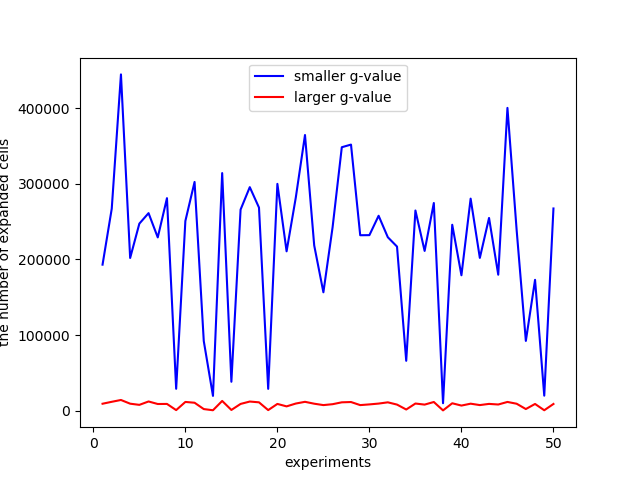
\includegraphics[scale = 0.3]{smaller_g_and_larger_g.png}
	\caption{Smaller g-value and larger g-value}
	\label{fig:Fig2.S&L}
\end{figure}
\newline
According to the result, we can find that the number of expanded cells of mode=0 is always bigger than the number of expanded cells of mode=1, which means the Repeated Forward A* using larger g-value tie breaking strategy is faster than Repeated Forward A* using smaller g-value tie breaking strategy.\\
The reason is that the agent will choose the point closer to the target to expand if we choose larger g-value to break ties. For two cells $s_1$, $s_2$ with f-value $f(s_1)=f(s_2)$, if $$g(s_1)>g(s_2)$$
then
	$$h(s_1) = f(s_1) - g(s_1)
	\leq f(s_2) - g(s_2)
	=h(s_2)$$ 
Therefore, if the A* use larger g-value to break tie, it will choose a cell with smaller h-value, which is closer to the goal. In A* searching, all cells with $f$ smaller than $gd(start)$ will be expanded. So, the breaking ties strategy only affect how many cells with $f = gd(start)$ will be expanded. If A* choose to expand a cell with smaller g-value, it will expand almost all the cells with $f = gd(start)$ before it add $goal$ to the open list.
%Thus, we choose the state with larger h-value to expand, which means we choose to expand the state that is closer to the start states and expand all other states with the same f-value and g-value as $s_1$ before  we can expand the states with the same f-value but with smaller h-value in this case. Similarly, for mode 1 we choose larger g-value to break tie, which means we choose $s_2$ to expand. Because $h(s_1)>h(s_2)$, we choose the point that is closer to the target in this case and don't need to expand any other states that have the same f-value and g-value with $s_2$ before we expand the state with the same f-value but smaller h-value.  
Let's consider the following example to see which cells the two modes will choose to expand.
\begin{figure}[htb]
	\centering
	\subfigure[maze]{
	\label{fig:Fig2.exp}
	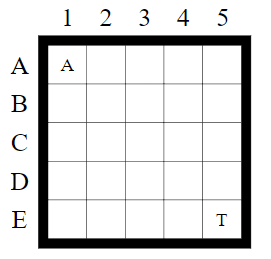
\includegraphics[width=3cm, height=2.89cm]{part2_example.png}}
	\subfigure[smaller]{
	\label{fig:Fig2.smaller}
	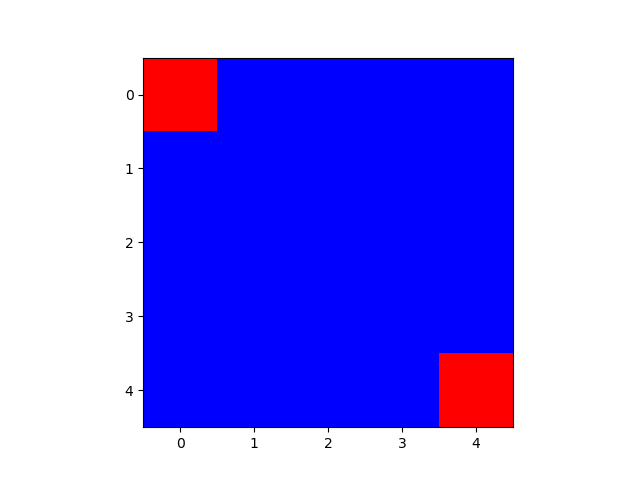
\includegraphics[scale = 0.2]{smaller_g}}
	\subfigure[larger]{
	\label{fig:Fig2.larger}
	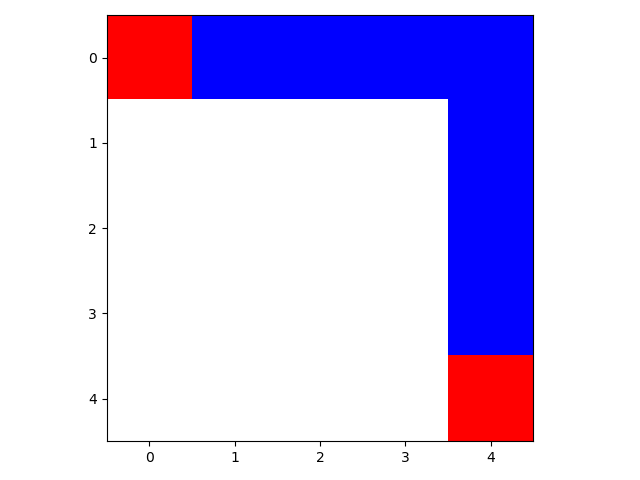
\includegraphics[scale = 0.2]{larger_g}}
	\caption{Expanded map}
\end{figure}
\newline 
For mode 0, see Fig. \ref{fig:Fig2.larger}.
The cells in blue means that the cells have been expanded through the whole search process.\\ 
For mode 1, see Fig. \ref{fig:Fig2.smaller}.\\
From these two results, we can see that we expand the cells closer and closer to the target when we choose larger g-value but we expand all the cells when we choose smaller larger g-value. 
\newline 
For mode 0(smaller g-value to break tie), here is the order of expansion,
\newline(we always choose the point that is put into the open list earlier to expand when both f-value and g-value are equal).
$$A1$$
$$\to A2\to B1$$
$$\to A3\to B2\to C1$$
$$\to A4\to B3\to C2\to D1$$
$$\to A5\to B4\to C3\to D2\to E1$$
$$\to B5\to C4\to D3\to E2$$
$$\to C5\to D4\to E3$$
$$\to D5$$
All the cells in this maze have same f-value. The level from high to low correspond the g-value from large to small.
\newline
For mode 0, we can see that the algorithm first expand all cells with smallest g-values, and then the second smallest and so on. Before it reach the goal, the algorithm have expand almost all cells in maze. That is far inefficient than mode 1. 
Here is the order of the expansion of the cells for mode 1,
$$A1\to A2\to A3\to A4\to A5\to B5\to C5\to D5$$
We can see that the algorithm only expand 1 cell in each level. The number of total expended cells is less than mode0.

%----------------------------------------------------------------------------------------

\section*{part 3}
The Repeated Forward A* and Repeated Backward A* can share same A* searching algorithm. Therefore, to implement these 2 algorithm, we add a parameter $decode_{mode}$ to our A* function. When $decode_{mode} = 1$, the function will swap the position of $start$ and $goal$ and invert the $path$ to do Backward A* searching.
	\begin{figure}[htb]
		\centering
		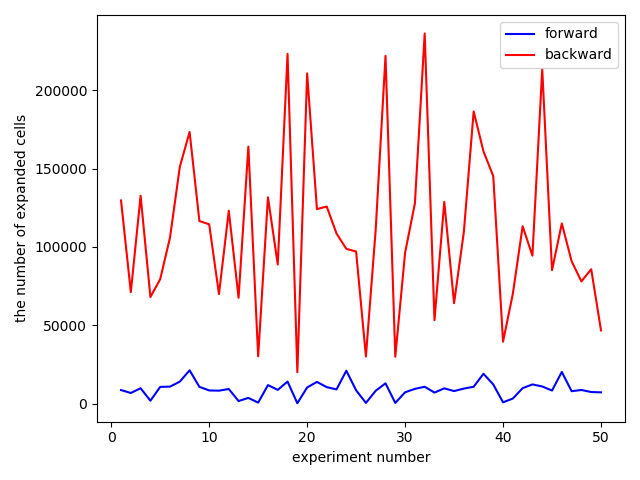
\includegraphics[scale = 0.3]{forward_backward.png}
		\caption{Forward A* search and Backward A* search}
		\label{fig:Fig3.F&B}
	\end{figure}
\newline
Fig. \ref{fig:Fig3.F&B} shows the result of 50 test on $101\times 101$ maze. According to the  result, Repeated Forward A* expanded much less  nodes than Repeated Backward A*. On average, Repeated Forward A* only expand $9113$ nodes in each test, whereas Repeated Backward A* expand $111250$ nodes. In addition, the variance of Repeated Forward A* is $24296811$, and the variance of Repeated Backward A* is $2758697079$. So, Repeated Forward A* is also more stable than Repeated Backward A*.
\newline
The reason is that the known world is closer to $start$ than $goal$. In general, for any two points, if there are more blocked cells around one point, the cost of the path between them will be expectedly higher. Since the known world is closer to $start$, the blocked cells are relatively close to $start$. Therefore, for any two cells $a$ and $b$ respectively in forward and backward search, if $h(a) = h(b)$, there are higher probability that $g(a) > g(b)$. So, in general, there are more cells $s$ with $f(s) < gd(start)$ in backward a* search than in forward a* search. Since all cells with $f(s) < gd(start)$ will be expanded in A* search, Backward A* search will expand more cells.



%----------------------------------------------------------------------------------------

\section*{Part 4}



%------------------------------------------------

\subsection*{Proving Manhattan distances are consistent:}

According to triangle inequality, for any three point $a, b$ and $c$, we have
	$$h(a, c) \leq h(a, b) + h(b, c)$$
$h(a, c)$ is the Manhattan distance between $a$ and $c$.
\newline
Then, since the agent can move only in the four main compass directions, the shortest distant between any two points is their Manhattan distances. So,
	$$h(a, b) + h(b, c)\leq c(a, b) + h(b, c)$$
$c(a, b)$ is the real distance between $a$ and $b$. So, any two point $a$ and $b$ satisfy
	$$h(a, c) \leq c(a, b) + h(b, c)$$
Therefore, Manhattan distance are consistent.

\subsection*{Proving Adaptive A* is constances}

Proving by induction.
\newline
Since the initially h-values are consistent, we assume the h-values in first $i-1$ searching are consistent, and need to prove the h-values in $i^{th}$ searching are consistent. Separating the situation of any two cell $a$ and $b$ into three cases and prove
	$$h^i(a)\leq c^i(a, b) + h^i(b)$$
\begin{enumerate}
	\item Both $a$ and $b$ were expanded in ${i-1}^{th}$ search.
\newline Because both $a$ and $b$ were expanded, their h-values in $i^{th}$ search are
$$h^i(a)=g^{i-1}(goal)-g^{i-1}(a) 
\text{ and }
h^i(b)=g^{i-1}(goal)-g^{i-1}(b)$$
According to triangle inequality, we know
$$g^{i-1}(b)\leq g^{i-1}(a)+c^{i-1}(a,b)$$
Therefore, because the action cost is nondecreasing
\begin{equation}\nonumber
\begin{aligned}
h^i(a)&=g^{i-1}(goal)-g^{i-1}(a)\\ &\leq g^{i-1}(goal)-g^{i-1}(a)+c^{i}(a,b)\\&\leq h^{i}(b)+c^i(a,b)
\end{aligned}
\end{equation}

\item $a$ was expanded but $b$ was not.\\
Because $a$ was expanded but $b$ wasn't, their h-values in $i^{th}$ search are
$$h^i(a)=g^{i-1}(goal)-g^{i-1}(a) 
\text{ and }
h^i(b)=h^{i-1}(b)$$
According to triangle inequality, we know
$$g^{i-1}(b)\leq g^{i-1}(a)+c^{i-1}(a,b)$$
Because $b$ wasn't expanded, according to the expanding rule of A*, we have
$$g^{i-1}(goal)\leq g^{i-1}(b) + h^{i-1}(b)$$
Therefore,
\begin{equation}\nonumber
\begin{aligned}
h^i(a)&=g^{i-1}(goal)-g^{i-1}(a)\\ &\leq g^{i-1}(b) + h^{i-1}(b) - g^{i-1}(a)\\&\leq h^{i}(b)+c^i(a,b)
\end{aligned}
\end{equation}

\item $b$ was expanded but $a$ wasn't expanded.
\newline In this case, 
$$h^i(a)=h^{i-1}(a) 
\text{ and }
h^i(b)=g^{i-1}(goal)-g^{i-1}(b)$$
Because the heuristic action cost keeps nondecreasing, we can know 
$$h^i(a)=h^{i-1}(s)\leq h^{i-1}(b)+c^{i-1}(a,b)\leq h^{i}(b)+c^{i}(a,b)$$ 
\end{enumerate}
Therefore, we prove that Adaptive A* leaves initially consistent h-values consistent 

\section*{Part 5}
Fig. \ref{fig:Fig5.ada} shows the result of 50 independent tests for repeated A* search and adaptive A*.
\begin{figure}[htb]
	\centering
	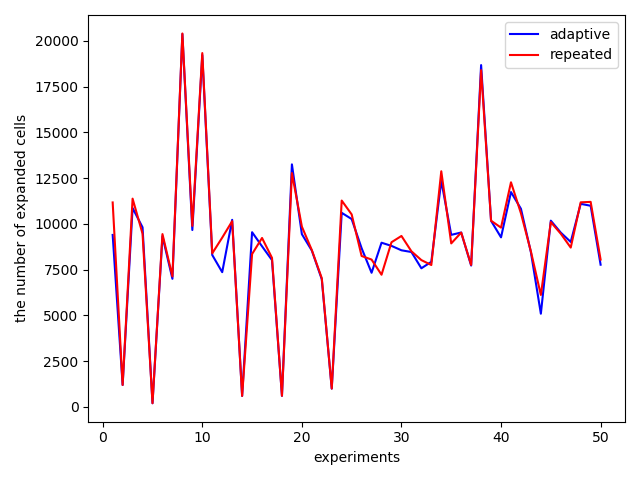
\includegraphics[scale = 0.3]{repeated_adaptive.png}
	\caption{Repeated A* and Adaptive A*}
	\label{fig:Fig5.ada}
\end{figure}
\newline
From this result figure, we can find the total expanded states of these two different searching algorithm is nearly equal but adaptive A* search expands a little less states than repeated A* search. The reason is that adaptive A* search use $h_{new}(s) = g(goal) - g(s)$ to update the h-value of all expanded cell $s$. Since we know that $gd(s)\geq h_{new}\geq h(s)$, the $h_{new}$ is more informed than the Manhattan distance $h(s)$. Therefore, Adaptive A* searching will expand less wrong cells (the cells out of the path) to find the path from $start$ to $goal$. 

%----------------------------------------------------------------------------------------
\section*{part 6}
Take the experiment question in part 2 to do a statistical hypothesis test.
\newline
Assume that performance differences between two search algorithms  are  due to sampling noise(null hypothesis). The probability of one algorithm performs better than another due to sampling noise is 50\%. Set the significance level of the test $\alpha=0.01$. The probability of getting the result in part 2 that the performance of breaking tie with larger g-value is better than the performance of breaking tie with smaller g-value shows up for 50 times in 50 experiments is $p=0.5^{50}<\alpha$, which is in the region of rejection, so we need to reject the null hypothesis. Therefore, performance differences between two search algorithms are systematic in nature but not due to sampling noise.


\end{document}